\documentclass{beamer}
\usepackage{alltt}
\usepackage{verbatim}
\usepackage{graphicx}

\usepackage{tikz}
\usepackage{svg}

\newcommand{\bs}{\symbol{`\\}}
\newcommand{\arr}{$\rightarrow$}
\newcommand{\LAMT}[1]{/\bs{}{#1} \arr }
\newcommand{\lam}[1]{\bs{}{#1} \arr }
\newcommand{\bl}[1]{\textcolor[rgb]{0.0,0.5,0.9}{#1}}
\newcommand{\g}[1]{\textcolor[rgb]{0.7,0.3,0.3}{#1}}
\newcommand{\off}[1]{\textcolor[rgb]{0.7,0.7,0.7}{#1}}

\begin{document}
\title{Rate inference for flow fusion}
\author{Amos Robinson\\PhD student at UNSW}

\frame{\titlepage}

\begin{frame}[fragile]{\emph{Shortcut fusion} is great, but\ldots}
\begin{itemize}
\item Relies on inlining - depends on compiler's mood
\item `Local' - only looks at a few combinators at a time
\item User must inspect core to find out whether it all fused
\end{itemize}
\end{frame}


\begin{frame}[fragile]{\emph{Flow fusion} is a more global transform}
\begin{itemize}
\item Being implemented as a GHC compiler plugin
\item Core operation fuses set of combinators into single loop, if possible
\item I imagine most of you have seen Ben's talk on this
\end{itemize}
\end{frame}


\begin{frame}{\emph{Rate inference} schedules combinators into groups}
\begin{itemize}
\item Each group becomes a single loop
\item Aim to minimise number of loops and number of buffers
\item This is what I'm talking about
\end{itemize}
\end{frame}


\begin{frame}[fragile,b]{Construct graph}
\begin{itemize}
\item Combinators are nodes
\item Folds need all input before producing, so edge is \emph{fusion-preventing}
\end{itemize}

\begin{columns}
\column[t]{5cm}

\begin{alltt}\small
filterMax (\bl{vs} : Vector Int) =
 let vs' = \g{map}    (+1)    vs
     m   = \g{fold}     0 max vs'
     vs''= \g{filter} (>0)    vs'
 in (\bl{m}, \bl{vs''})
\end{alltt}

\column[t]{5cm}

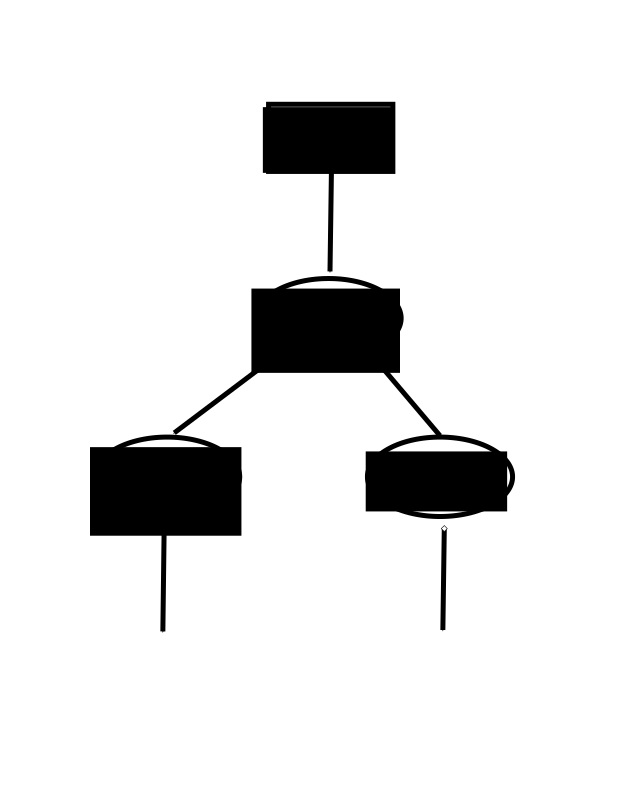
\includegraphics[scale=0.5]{gen/filterMax-unfused.png}

\end{columns}
\end{frame}


\begin{frame}[fragile,b]{Size/rate annotation}
\begin{itemize}
\item Give each input fresh rate variable and propagate
\item Filters are of \emph{unknown} length \\ with some upper bound
\end{itemize}


\begin{columns}
\column[t]{5cm}

\column[t]{5cm}

\includegraphics[scale=0.5]{gen/filterMax-rates.png}

\end{columns}
\end{frame}


\begin{frame}[fragile,b]{Scheduling}
Finding a minimal schedule for this case is easy
\begin{itemize}
\item Souces are 0
\item $w(v) = \max_u (w(u) + \delta(u,v))$
\item $\delta(edge) = 1$ if edge is fusion preventing
\end{itemize}


\begin{columns}
\column[t]{5cm}

\column[t]{5cm}

\includegraphics[scale=0.5]{gen/filterMax-schedule0.png}

\end{columns}
\end{frame}

\begin{frame}[fragile,b]{Scheduling}
Finding a minimal schedule for this case is easy
\begin{itemize}
\item Souces are 0
\item $w(v) = \max_u (w(u) + \delta(u,v))$
\item $\delta(edge) = 1$ if edge is fusion preventing
\end{itemize}


\begin{columns}
\column[t]{5cm}

\column[t]{5cm}

\includegraphics[scale=0.5]{gen/filterMax-schedule1.png}

\end{columns}
\end{frame}


\begin{frame}[fragile,b]{Minimal buffers}
Some cases aren't quite as easy to schedule

\begin{columns}
\column[t]{5cm}

\begin{alltt}
normalise (\bl{vs} : Vector Int) =
 let m   = \g{fold}     0 sum vs'
     vs' = \g{map}    (+1)    vs
     vs''= \g{map}    (/m)    vs'
 in (\bl{vs''})
\end{alltt}

\column[t]{5cm}

\includegraphics[scale=0.5]{gen/normalise-unfused.png}

\end{columns}
\end{frame}

\begin{frame}[fragile,b]{Minimal buffers}
This scheduling requires a buffer for the first map's output.

\begin{columns}
\column[t]{5cm}

\column[t]{5cm}

\includegraphics[scale=0.5]{gen/normalise-schedule.png}

\end{columns}
\end{frame}


\begin{frame}[fragile,b]{Minimal buffers}

\begin{itemize}
\item The existing schedule is the \emph{earliest}
\item Working backwards, create a \emph{latest} schedule
\item $w(v) = \min_u (w(u) - \delta(u,v))$
\end{itemize}

\begin{columns}
\column[t]{5cm}

\column[t]{5cm}

\includegraphics[scale=0.5]{gen/normalise-latest.png}

\end{columns}
\end{frame}


\begin{frame}[fragile,b]{Minimal buffers}

\begin{itemize}
\item The \emph{optimal} schedule is somewhere in between
\item The optimal schedule minimises edge crossings
\item (In this case it is the same as the latest schedule)
\end{itemize}

\begin{columns}
\column[t]{5cm}

\column[t]{5cm}

\includegraphics[scale=0.5]{gen/normalise-optimal.png}

\end{columns}
\end{frame}

\begin{frame}[fragile,b]{Minimal buffers}

\begin{itemize}
\item The \emph{optimal} schedule is somewhere in between
\item The optimal schedule minimises edge crossings
\item (In this case it is the same as the latest schedule)
\end{itemize}

\begin{columns}
\column[t]{5cm}

\column[t]{5cm}

\includegraphics[scale=0.5]{gen/normalise-optimalsched.png}

\end{columns}
\end{frame}


\begin{frame}[fragile,b]{Mixing sizes}
Combinators of different sizes cannot be fused

\begin{columns}
\column[t]{5cm}

\column[t]{5cm}

\includegraphics[scale=0.5]{gen/types-unfused.png}

\end{columns}
\end{frame}


\begin{frame}[fragile,b]{Mixing sizes}
\begin{itemize}
\item Perform scheduling for each size variable separately
\item With a slightly different $\delta$ function:
\item $\delta(edge) = 1$ if edge is fusion preventing and source is same type
\end{itemize}

\begin{columns}
\column[t]{5cm}

\column[t]{5cm}

\includegraphics[scale=0.5]{gen/types-schedule.png}

\end{columns}
\end{frame}


\begin{frame}[fragile,b]{Mixing sizes}
\begin{itemize}
\item Merge fusible nodes of given type together
\end{itemize}

\begin{columns}
\column[t]{5cm}

\column[t]{5cm}

\includegraphics[scale=0.5]{gen/types-schedule1.png}

\end{columns}
\end{frame}


\begin{frame}[fragile,b]{Mixing sizes}
\begin{itemize}
\item Scheduling next type on merged graph
\end{itemize}

\begin{columns}
\column[t]{5cm}

\column[t]{5cm}

\includegraphics[scale=0.5]{gen/types-schedule2.png}

\end{columns}
\end{frame}


\begin{frame}[fragile,b]{Mixing sizes}
\begin{itemize}
\item After all types are done, we end up with
\end{itemize}

\begin{columns}
\column[t]{5cm}

\column[t]{5cm}

\includegraphics[scale=0.5]{gen/types-schedule3.png}

\end{columns}
\end{frame}


\begin{frame}[fragile,b]{Filters}
\begin{itemize}
\item Filters are special
\item Despite being different sizes, they \emph{can} be fused into their parents
\item I'm still not sure about the best way to do this
\end{itemize}

\begin{columns}
\column[t]{5cm}

\column[t]{5cm}

\includegraphics[scale=0.5]{gen/filter3-fused.png}

\end{columns}
\end{frame}


\begin{frame}[fragile]{The end}
thanks
\end{frame}


\begin{frame}[fragile]{Size/rate annotation redux}
It's a touch more complicated, but pretty boring:
\begin{itemize}
\item map2 (zipWith) requires inputs to be same rate
\item filters are \emph{skolem} and can't be constrained
\end{itemize}
\end{frame}

\end{document}
